\documentclass[tikz,border=2pt]{standalone}
\usepackage{amsmath}
\usetikzlibrary{arrows.meta}
\begin{document}
% Balking with K=4, lambda=1, mu=3: entry rates lambda^+(n)=lambda(K-n)=4,3,2,1,0 (blue)
% against blocking lambda 1{n<K} at the same potential rate 4 (grey dashed);
% stationary probabilities p(n)=(27,36,36,24,8)/131 (green).
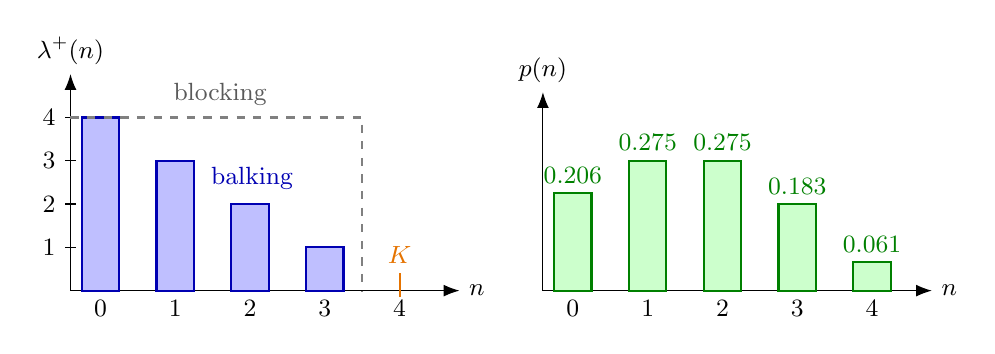
\begin{tikzpicture}[font=\small, >={Latex[length=2mm]}, x=0.95cm]
  % left panel: entry rates, 0.55 cm per unit
  \begin{scope}[y=0.55cm]
    \draw[->] (-0.4,0) -- (4.8,0) node[right] {$n$};
    \draw[->] (-0.4,0) -- (-0.4,5.0) node[above] {$\lambda^{+}(n)$};
    \foreach \y in {1,2,3,4} \draw (-0.47,\y) -- (-0.33,\y) node[pos=0, left] {$\y$};
    \foreach \n/\r in {0/4,1/3,2/2,3/1} {
      \fill[blue!25] (\n-0.25,0) rectangle (\n+0.25,\r);
      \draw[blue!70!black, thick] (\n-0.25,0) rectangle (\n+0.25,\r);
    }
    \foreach \n in {0,1,2,3,4} \node[below] at (\n,0) {$\n$};
    \draw[gray, thick, dashed] (-0.4,4) -- (3.5,4) -- (3.5,0);
    \node[gray!70!black, anchor=south] at (1.6,4.05) {blocking};
    \node[blue!70!black, anchor=west] at (1.35,2.6) {balking};
    \draw[orange!90!black, thick] (4,-0.15) -- (4,0.4);
    \node[orange!90!black, anchor=south] at (4,0.4) {$K$};
  \end{scope}
  % right panel: p(n), 6 cm per unit probability
  \begin{scope}[xshift=6.0cm, y=6cm]
    \draw[->] (-0.4,0) -- (4.8,0) node[right] {$n$};
    \draw[->] (-0.4,0) -- (-0.4,0.42) node[above] {$p(n)$};
    \foreach \n/\p in {0/0.206,1/0.275,2/0.275,3/0.183,4/0.061} {
      \fill[green!20] (\n-0.25,0) rectangle (\n+0.25,\p);
      \draw[green!50!black, thick] (\n-0.25,0) rectangle (\n+0.25,\p);
      \node[green!50!black, anchor=south] at (\n,\p) {$\p$};
      \node[below] at (\n,0) {$\n$};
    }
  \end{scope}
\end{tikzpicture}
\end{document}
